\subsection{The computer time}


\begin{table}[H]\caption{This is a table listing the computing time for each algorithm. The LU algorithm was only possible to do up till $ n=1e4 $ and the entry of 0 s means that this algorithm did not compute anything for the given value of n}
	\label{tab:time}
	\begin{tabular}{cccc}
		n & general($ s$)  & special($ s$) & LU(s)  \\ 
\hline  
1e1    &         1.5e-05      &       2.0e-06  &1.8e-04\\ 
1e2    &         1.9e-05      &       5.0e-06  &2.6e-03\\ 
1e3    &         4.8e-05      &       4.1e-05  &2.7e-01\\ 
1e4    &         5.9e-04      &       3.3e-04  &1.4e+02\\ 
1e5    &         5.2e-03      &       3.2e-03  &0.0e+00\\ 
1e6    &         6.6e-02      &       4.0e-02  &0.0e+00\\ 
1e7    &         5.8e-01      &       3.9e-01  &0.0e+00\\ 

	\end{tabular}
\end{table}

In the discussion section we will discuss the number of Floating Point Operations (FLOPS). There is however a limitation in the physical memory of the computer, which only allows us to create a certain size of matrix. Turns out we were not able to use the LU decomposition on the system for $ n> 1e4 $ matrixes on the form  $ n\times n $. Therefore there is no CPU-time for this algorithm. 

It is also clear to see that the special algorithm is significantly quicker compared to the other algorithms, see section \ref{section:FLOPS}. 

\subsection{Nummerical precision}


The relative error for the different values of h is represented in table \ref{tab:error_developement}. As these numbers are the maximum relative error of the entire matrix and does not represent a specific value of x. In order to generate the table we had to choose between the general and the special algorithm. As the special algorithm does not need to refer to a stored double in the script, but rather depends directly on h and an integer, this yields a smaller relative error for the smaller values of h compared to the general algorithm. 

We can see that the smallest error, $log_{10}(RelativeError) = -10.15$, is accomplished for  $ h = 1\E{-6} $. As h decreases further, numerical round-off-errors become significant and the relative error increases. 


\begin{table}[H]\caption{Maximum relative error ($ \epsilon $) for a given value of h. Both the special algorithm and the general was used to generate this table.} \label{tab:error_developement}
	\begin{tabular}{ccc}
		$ \log_{10}$(h) &   $ \epsilon_{Max}$ , general $\epsilon_{Max} $, special\\ 
\hline  
-1 & -1.18 & -1.18 \\ 
-2 & -3.09 & -3.09 \\ 
-3 & -5.08 & -5.08 \\ 
-4 & -7.08 & -7.08 \\ 
-5 & -8.84 & -9.08 \\ 
-6 & -6.08 & -10.16 \\ 
-7 & -5.53 & -9.09 \\ 

	\end{tabular}
\end{table}

For high values of $ h $, numerical errors is not important and both the special and general algorithm gives similar errors.Therefore, the data plotted in figures \ref{fig:num1e1} and \ref{fig:num1e3} comes from the special algorithm. For high values of h, as in figure \ref{fig:num1e1}, the absolute error is significantly greater than for lower values of h, see figure \ref{fig:num1e3}.  

\begin{figure}[H]
	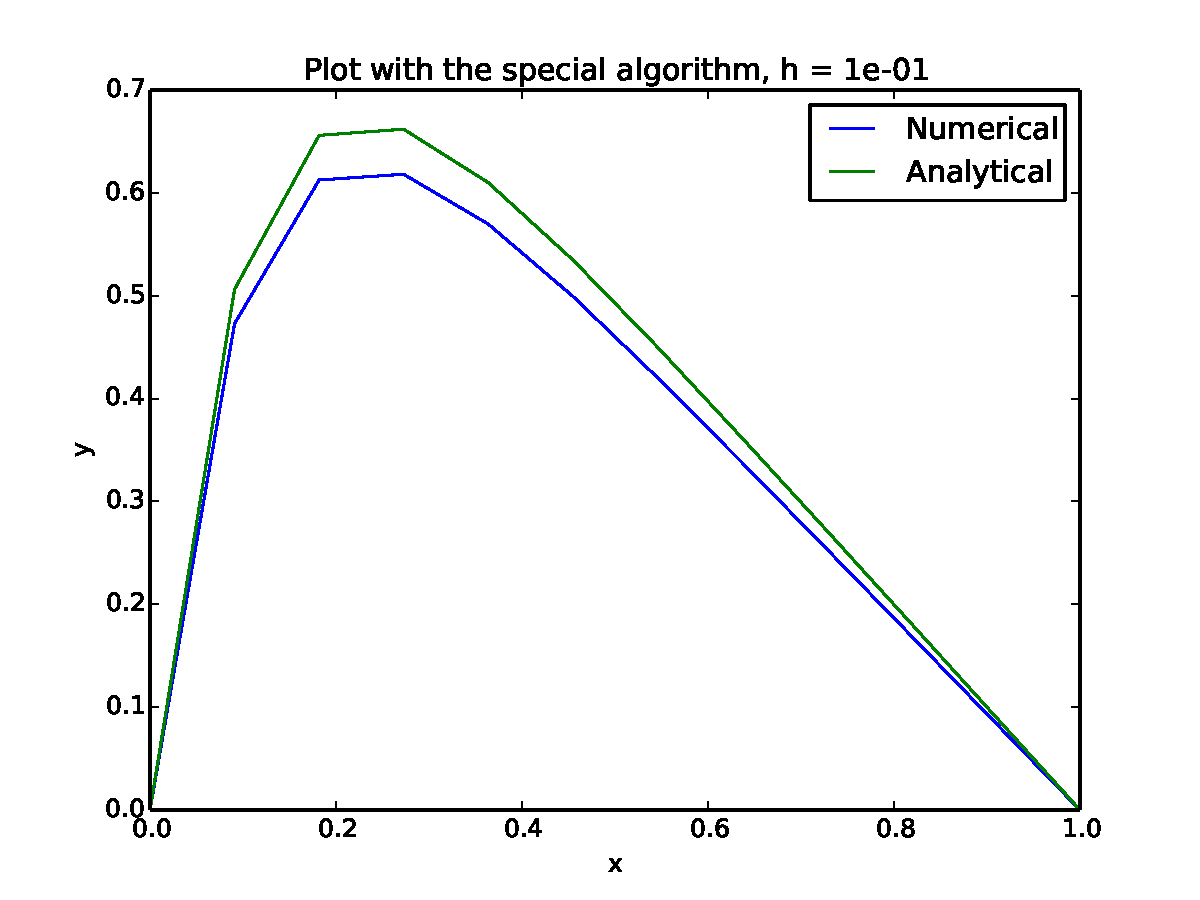
\includegraphics[width = 1 \linewidth]{../programs/Plotting_kjetil/n_10.pdf}
	\caption{Plot of the results using the special algorithm comparing the numerical and analytical result for a $ 10\times 10 $ matrix. The  nummerical solution is significantly different from the analytical one.}
	\label{fig:num1e1}
\end{figure}


\begin{figure}[H]
	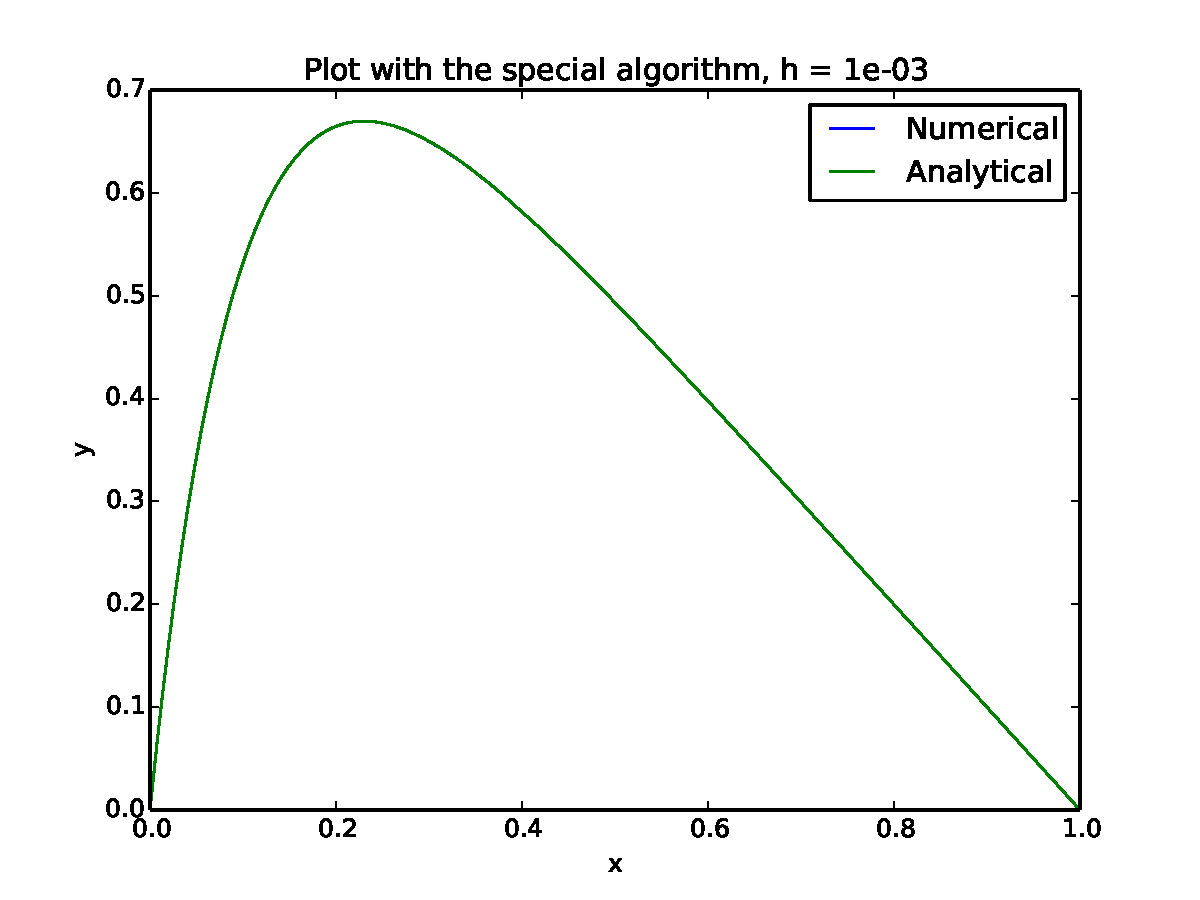
\includegraphics[width = 1 \linewidth]{../programs/Plotting_kjetil/n_1000.pdf}
	\caption{Plot of the results using the special algorithm comparing the numerical and analytical result for a $ 1e3\times 1e3 $ matrix. The errors are now impossible to see in this plot}
	\label{fig:num1e3}
\end{figure}





